\documentclass{article}
\usepackage[utf8]{inputenc}
\usepackage{hyperref}
\usepackage{listings}
\usepackage{xcolor}
\usepackage[margin=1in]{geometry}
\usepackage{tikz}
\usepackage{booktabs}
\usepackage{longtable}
\usepackage{array}
\usepackage{enumitem}
\usepackage{fancyhdr}
\usepackage{titlesec}
\usetikzlibrary{shapes.geometric, arrows.meta, positioning, fit, backgrounds}

% --- Colour palette ------------------------------------------------------------
\definecolor{codegreen}{rgb}{0,0.6,0}
\definecolor{codegray}{rgb}{0.5,0.5,0.5}
\definecolor{codepurple}{rgb}{0.58,0,0.82}
\definecolor{backcolour}{rgb}{0.95,0.95,0.92}
\definecolor{evblue}{RGB}{30,100,200}
\definecolor{emsgreen}{RGB}{20,140,80}
\definecolor{cargoamber}{RGB}{200,120,0}
\definecolor{rowgray}{gray}{0.92}

% --- Listing style -------------------------------------------------------------
\lstdefinestyle{mystyle}{
    backgroundcolor=\color{backcolour},
    commentstyle=\color{codegreen},
    keywordstyle=\color{magenta},
    numberstyle=\tiny\color{codegray},
    stringstyle=\color{codepurple},
    basicstyle=\ttfamily\footnotesize,
    breakatwhitespace=false,
    breaklines=true,
    captionpos=b,
    keepspaces=true,
    numbers=left,
    numbersep=5pt,
    showspaces=false,
    showstringspaces=false,
    showtabs=false,
    tabsize=2,
}
% Define JSON as a listings language
\lstdefinelanguage{json}{
    morestring=[b]",
    morecomment=[l]{//},
    sensitive=false,
}

\lstset{style=mystyle}

% --- HTTP method macros --------------------------------------------------------
\newcommand{\GET}{\colorbox{evblue!20}{\texttt{\textbf{\color{evblue}GET}}}}
\newcommand{\POST}{\colorbox{emsgreen!20}{\texttt{\textbf{\color{emsgreen}POST}}}}
\newcommand{\PUT}{\colorbox{cargoamber!20}{\texttt{\textbf{\color{cargoamber}PUT}}}}
\newcommand{\DELETE}{\colorbox{red!15}{\texttt{\textbf{\color{red}DELETE}}}}

% --- Page header ---------------------------------------------------------------
\pagestyle{fancy}
\fancyhf{}
\rhead{SIAM EV Platform --- API Reference}
\lhead{\leftmark}
\rfoot{Page \thepage}
\renewcommand{\headrulewidth}{0.4pt}

\hypersetup{
    colorlinks=true,
    linkcolor=evblue,
    urlcolor=evblue,
    pdftitle={SIAM EV Platform API Reference},
    pdfauthor={Ruslee Sutthaweekul}
}

% --- Document ------------------------------------------------------------------
\title{%
    \textbf{SIAM EV Platform}\\[6pt]
    \large API Reference\\
    \normalsize OCPP Charging Monitoring \textbullet\
    Energy Management System \textbullet\
    Cargo Space Monitoring
}
\author{Ruslee Sutthaweekul}
\date{Version 1.0 \quad\textbullet\quad \today}

\begin{document}

\maketitle
\tableofcontents
\newpage

% ==============================================================================
\section{Introduction}
% ==============================================================================

This document describes the REST and WebSocket APIs exposed by the SIAM EV Unified
Energy \& Logistics Management Platform. Three sub-systems are covered:

\begin{enumerate}
    \item \textbf{OCPP Charging Monitoring} --- real-time telemetry, remote commands,
          and scheduling for EV charging stations (OCPP 2.0.1).
    \item \textbf{Energy Management System (EMS)} --- facility-level energy analytics,
          demand-response controls, and renewable-source integration.
    \item \textbf{Cargo Space Monitoring} --- container/cargo-bay occupancy, temperature
          and humidity telemetry, and access-event logging for logistics hubs.
\end{enumerate}

\subsection{Base URL}

All endpoints are served under the API Gateway. Replace \texttt{\{host\}} with the
deployment address (e.g.\ \texttt{api.siam-ev.example.com}).

\begin{lstlisting}[language=bash, caption=Base URL pattern]
https://{host}/api/v1
\end{lstlisting}

\subsection{Authentication}

Every request must carry a Bearer token obtained from the Auth Service.

\begin{lstlisting}[language=bash, caption=Authorization header]
Authorization: Bearer <access_token>
\end{lstlisting}

\begin{center}
\begin{tabular}{>{\ttfamily}lll}
\toprule
\textbf{Header} & \textbf{Required} & \textbf{Description}\\
\midrule
Authorization & Yes & \texttt{Bearer <JWT>} issued by \texttt{/auth/token}\\
Content-Type  & Yes (POST/PUT) & \texttt{application/json}\\
X-Request-ID  & No  & Idempotency key; echoed in response headers\\
\bottomrule
\end{tabular}
\end{center}

\subsection{Common Error Schema}

\begin{lstlisting}[language=json, caption=Error response envelope]
{
  "success": false,
  "error": {
    "code": "STATION_NOT_FOUND",
    "message": "No station with id 'station-bkk-099' exists.",
    "timestamp": "2026-07-02T10:15:30Z"
  }
}
\end{lstlisting}

\begin{center}
\begin{tabular}{lll}
\toprule
\textbf{HTTP Status} & \textbf{Meaning} & \textbf{Common cause}\\
\midrule
200 & OK & Successful read\\
201 & Created & Resource created\\
400 & Bad Request & Missing or invalid fields\\
401 & Unauthorized & Missing / expired token\\
403 & Forbidden & Insufficient role\\
404 & Not Found & Resource does not exist\\
409 & Conflict & Duplicate resource\\
500 & Internal Error & Upstream / database failure\\
\bottomrule
\end{tabular}
\end{center}

\subsection{System Architecture Overview}

\begin{figure}[h]
\centering
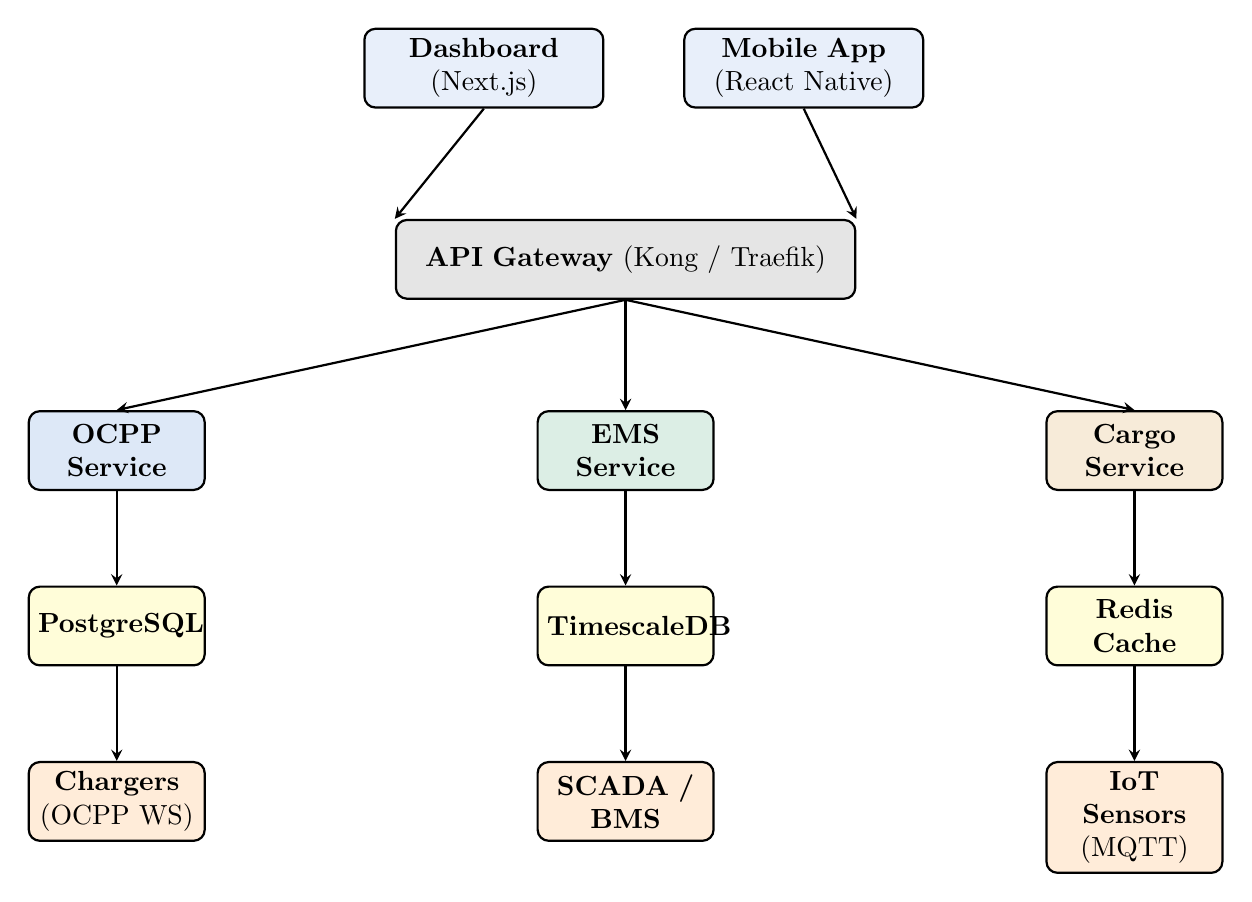
\begin{tikzpicture}[node distance=1.8cm and 2.4cm,
    box/.style={rectangle, rounded corners, minimum width=3cm, minimum height=1cm,
                text centered, text width=2.8cm, draw=black, thick, fill=gray!10},
    sbox/.style={box, minimum width=2.2cm, text width=2cm},
    arrow/.style={thick,->,>=stealth}]

% Client layer
\node (ui)  [box, fill=evblue!10]  {\textbf{Dashboard}\\ (Next.js)};
\node (mob) [box, fill=evblue!10, right=1cm of ui] {\textbf{Mobile App}\\ (React Native)};

% Gateway
\node (gw) [box, fill=gray!20, below=1.4cm of ui, xshift=1.8cm, minimum width=5.8cm, text width=5.6cm]
    {\textbf{API Gateway} (Kong / Traefik)};

% Services
\node (ocpp) [sbox, fill=evblue!15,    below left=1.4cm and 2.4cm of gw]  {\textbf{OCPP\\Service}};
\node (ems)  [sbox, fill=emsgreen!15,  below=1.4cm of gw]                 {\textbf{EMS\\Service}};
\node (cargo)[sbox, fill=cargoamber!15,below right=1.4cm and 2.4cm of gw] {\textbf{Cargo\\Service}};

% Data stores
\node (pg) [sbox, fill=yellow!15, below=1.2cm of ocpp] {\textbf{PostgreSQL}};
\node (ts) [sbox, fill=yellow!15, below=1.2cm of ems]  {\textbf{TimescaleDB}};
\node (rd) [sbox, fill=yellow!15, below=1.2cm of cargo]{\textbf{Redis\\Cache}};

% External
\node (hw) [sbox, fill=orange!15, below=1.2cm of pg] {\textbf{Chargers}\\ (OCPP WS)};
\node (scada)[sbox,fill=orange!15,below=1.2cm of ts]  {\textbf{SCADA /\\BMS}};
\node (iot)  [sbox,fill=orange!15,below=1.2cm of rd]  {\textbf{IoT Sensors}\\ (MQTT)};

% Arrows -- clients to gateway
\draw [arrow] (ui.south)  -- (gw.north west);
\draw [arrow] (mob.south) -- (gw.north east);
% Gateway to services
\draw [arrow] (gw.south) -- (ocpp.north);
\draw [arrow] (gw.south) -- (ems.north);
\draw [arrow] (gw.south) -- (cargo.north);
% Services to data
\draw [arrow] (ocpp.south) -- (pg.north);
\draw [arrow] (ems.south)  -- (ts.north);
\draw [arrow] (cargo.south)-- (rd.north);
% Services to external
\draw [arrow] (pg.south)  -- (hw.north);
\draw [arrow] (ts.south)  -- (scada.north);
\draw [arrow] (rd.south)  -- (iot.north);
\end{tikzpicture}
\caption{SIAM EV Platform --- high-level integration architecture}
\end{figure}

\newpage

% ==============================================================================
\section{OCPP Charging Monitoring API}
% ==============================================================================

\textbf{Base path:} \texttt{/api/v1/ocpp}

This sub-system exposes real-time telemetry from EV charging stations and accepts
remote control commands conforming to OCPP 2.0.1. The backend implementation uses
Node-RED as the Central System (CS); see \texttt{OCPP\_NodeRED\_Implementation.pdf}
for the Node-RED flow details.

% --- 2.1 Data models ----------------------------------------------------------
\subsection{Data Models}

\subsubsection{Station Object}

\begin{lstlisting}[language=json, caption=Station object schema]
{
  "id":          "station-bkk-001",      // string  --- unique station identifier
  "name":        "Siam Paragon Hub",     // string
  "lat":         13.7462,               // number  --- latitude
  "lng":         100.5347,              // number  --- longitude
  "status":      "Available",           // enum    --- see Status Codes below
  "connectors": [                       // array   --- one entry per plug
    {
      "connectorId": 1,
      "type":        "CCS2",
      "maxPowerKw":  150,
      "status":      "Available"
    }
  ],
  "currentMeter":  42.15,              // number  --- session energy (kWh)
  "powerOutput":   68.4,               // number  --- live power draw (kW)
  "powerLimit":    120,                // number  --- configured cap (kW)
  "firmwareVersion": "2.1.4",          // string
  "lastHeartbeat": "2026-07-02T09:58:00Z", // ISO-8601
  "schedule": {
    "startTime": "18:00",              // HH:MM local
    "endTime":   "08:00",             // HH:MM local
    "enabled":   true
  }
}
\end{lstlisting}

\begin{center}
\begin{tabular}{ll}
\toprule
\textbf{status value} & \textbf{Meaning}\\
\midrule
\texttt{Available}   & Idle, ready to charge\\
\texttt{Preparing}   & EV plugged in, waiting for auth\\
\texttt{Charging}    & Active charging session\\
\texttt{SuspendedEV} & Car paused session\\
\texttt{Finishing}   & Session ending\\
\texttt{Faulted}     & Hardware fault\\
\texttt{Unavailable} & Station taken offline\\
\bottomrule
\end{tabular}
\end{center}

% --- 2.2 Endpoints ------------------------------------------------------------
\subsection{Endpoints}

\subsubsection{\GET\ \ \texttt{/ocpp/stations} --- List all stations}

Returns the current telemetry snapshot for every registered charging station.

\textbf{Query parameters:}

\begin{center}
\begin{tabular}{>{\ttfamily}llll}
\toprule
\textbf{Param} & \textbf{Type} & \textbf{Default} & \textbf{Description}\\
\midrule
status & string & --- & Filter by status enum value\\
limit  & integer & 100 & Max records returned\\
offset & integer & 0 & Pagination offset\\
\bottomrule
\end{tabular}
\end{center}

\textbf{Response 200:}
\begin{lstlisting}[language=json, caption=GET /ocpp/stations response]
{
  "success": true,
  "data": [ /* array of Station objects */ ],
  "meta": { "total": 12, "limit": 100, "offset": 0 }
}
\end{lstlisting}

\subsubsection{\GET\ \ \texttt{/ocpp/stations/\{id\}} --- Get single station}

\textbf{Path parameter:} \texttt{id} --- the station identifier string.

\textbf{Response 200:}
\begin{lstlisting}[language=json, caption=GET /ocpp/stations/{id} response]
{
  "success": true,
  "data": { /* Station object */ }
}
\end{lstlisting}

\textbf{Response 404:}
\begin{lstlisting}[language=json]
{ "success": false, "error": { "code": "STATION_NOT_FOUND", ... } }
\end{lstlisting}

\subsubsection{\POST\ \ \texttt{/ocpp/stations/\{id\}/command} --- Send remote command}

Dispatches an OCPP remote command to the station.

\textbf{Request body:}
\begin{lstlisting}[language=json, caption=Remote command request]
{
  "action": "RemoteStopTransaction",  // or RemoteStartTransaction | Reset | ...
  "payload": {
    "transactionId": 7841             // required for RemoteStopTransaction
  }
}
\end{lstlisting}

\textbf{Supported \texttt{action} values:}

\begin{center}
\begin{tabular}{ll}
\toprule
\textbf{action} & \textbf{Description}\\
\midrule
\texttt{RemoteStartTransaction} & Begin a charging session\\
\texttt{RemoteStopTransaction}  & Stop an active session\\
\texttt{Reset}                  & Reboot the charge point (\texttt{"Hard"} or \texttt{"Soft"})\\
\texttt{ChangeAvailability}     & Set connector to Available / Unavailable\\
\texttt{SetChargingProfile}     & Push a smart-charging profile (kW limit)\\
\bottomrule
\end{tabular}
\end{center}

\textbf{Response 200:}
\begin{lstlisting}[language=json, caption=Command accepted response]
{
  "success": true,
  "data": {
    "status": "Accepted",
    "action": "RemoteStopTransaction"
  }
}
\end{lstlisting}

\subsubsection{\PUT\ \ \texttt{/ocpp/stations/\{id\}/schedule} --- Update charging schedule}

Sets the time-window schedule for a station's smart-charging controller.

\textbf{Request body:}
\begin{lstlisting}[language=json, caption=Schedule update request]
{
  "startTime": "22:00",   // HH:MM --- begin off-peak window
  "endTime":   "06:00",   // HH:MM --- end off-peak window
  "enabled":   true
}
\end{lstlisting}

\textbf{Response 200:}
\begin{lstlisting}[language=json]
{ "success": true, "data": { "stationId": "station-bkk-001", "schedule": { ... } } }
\end{lstlisting}

% --- 2.3 WebSocket ------------------------------------------------------------
\subsection{WebSocket --- Live Telemetry Stream}

Connect to receive real-time telemetry push events without polling.

\begin{lstlisting}[language=bash, caption=WebSocket connection]
wss://{host}/api/v1/ocpp/ws?token=<access_token>
\end{lstlisting}

\textbf{Server-sent event (JSON frame):}
\begin{lstlisting}[language=json, caption=Telemetry push event]
{
  "event": "MeterValues",
  "stationId": "station-bkk-002",
  "data": {
    "connectorId":   1,
    "transactionId": 7841,
    "energy_kWh":    58.34,
    "power_kW":      72.1,
    "voltage_V":     400.2,
    "current_A":     180.1,
    "timestamp":     "2026-07-02T10:05:42Z"
  }
}
\end{lstlisting}

\textbf{Additional event types:}

\begin{center}
\begin{tabular}{ll}
\toprule
\textbf{event} & \textbf{Trigger}\\
\midrule
\texttt{StatusNotification}  & Station or connector status change\\
\texttt{HeartBeat}           & Periodic station heartbeat (every 60 s)\\
\texttt{StartTransaction}    & New session started\\
\texttt{StopTransaction}     & Session ended (includes final kWh)\\
\texttt{FirmwareStatusNotification} & OTA update progress\\
\bottomrule
\end{tabular}
\end{center}

\newpage

% ==============================================================================
\section{Energy Management System (EMS) API}
% ==============================================================================

\textbf{Base path:} \texttt{/api/v1/ems}

The EMS sub-system aggregates energy consumption data from buildings and facilities,
provides time-series analytics, and exposes demand-response controls. Data is
persisted in TimescaleDB and read from SCADA / BMS systems over Modbus TCP or MQTT.

\textbf{Relationship to Cargo Stations.}
Every truck station in the Cargo sub-system is also an EMS \emph{facility} --- they
are the same physical site viewed from two operational domains. A single shared
identifier (\texttt{site-bkk-001}) is used as both the \texttt{facilityId} in EMS
responses and the \texttt{stationId} in Cargo responses. The EMS facility object
therefore includes the list of cargo-bay zones it contains, and each EMS energy
reading can be scoped to an individual cargo bay via the zone-level endpoints
(Section~\ref{sec:ems-zones}).

% --- 3.1 Data models ----------------------------------------------------------
\subsection{Data Models}

\subsubsection{Facility Object}

\begin{lstlisting}[language=json, caption=Facility object schema]
{
  "id":           "site-bkk-001",       // shared key: facilityId in EMS = stationId in Cargo
  "name":         "Thai Post Sorting Hub --- Lad Krabang",
  "type":         "LogisticsWarehouse",  // Office | Retail | Warehouse | LogisticsWarehouse
  "location": {
    "lat": 13.7284,
    "lng": 100.7498,
    "address": "999 Moo 1, Lad Krabang, Bangkok 10520"
  },
  // --- EMS energy fields ---
  "ratedCapacityKva":    2000,
  "currentDemandKw":     312.4,
  "peakDemandKw":        1540.0,        // rolling 12-month peak
  "dailyEnergyKwh":      7820.5,
  "solarCapacityKw":     500,
  "batteryCapacityKwh":  1000,
  "batteryStateOfCharge": 0.78,         // 0.0--1.0
  "gridImportKw":        -45.2,         // negative = exporting to grid
  "demandResponseActive": false,
  "tariffZone":          "TOU-EV",
  // --- Cargo station cross-reference ---
  "cargoStation": {
    "stationId":       "site-bkk-001",  // same value; emphasises the shared identity
    "activeTrucks":    3,               // trucks currently at this station
    "cargoBayZones": [
      { "zoneId": "zone-site-001-cold-01", "name": "Cold Room A",
        "currentKw": 42.1, "occupancyPct": 68 },
      { "zoneId": "zone-site-001-bay-02",  "name": "Dry Bay 2",
        "currentKw":  8.3, "occupancyPct": 55 },
      { "zoneId": "zone-site-001-dock-03", "name": "Loading Dock 3",
        "currentKw": 12.7, "occupancyPct": 0  }
    ],
    "ocppStationIds":  ["station-bkk-001", "station-bkk-002"]  // EV chargers on-site
  },
  "updatedAt": "2026-07-02T10:00:00Z"
}
\end{lstlisting}

\subsubsection{Zone Object (EMS --- authoritative sensor record)}

A \emph{zone} is a named, bounded space inside a facility (cold room, loading dock,
dry-storage bay). All environmental sensor data for zones is owned by EMS and read
from the facility's BMS or SCADA system over Modbus TCP or MQTT.
The Cargo sub-system does \textbf{not} maintain its own sensor pipeline for fixed
spaces --- it reads zone data from these EMS endpoints.

\begin{lstlisting}[language=json, caption=EMS zone object schema]
{
  "zoneId":      "zone-site-001-cold-01",
  "facilityId":  "site-bkk-001",
  "name":        "Cold Room A",
  "type":        "ColdRoom",            // ColdRoom | LoadingDock | DryBay | StagingArea
  // --- Energy (from SCADA / smart sub-meter) ---
  "currentKw":   42.1,
  "dailyKwh":    892.6,
  // --- Environment (from BMS sensors) ---
  "environment": {
    "temperatureC": 3.8,               // null if no temp sensor
    "humidityPct":  84.1,
    "co2Ppm":       405,
    "lightLux":     0
  },
  "setpointC":   4.0,                  // BMS setpoint (ColdRoom only)
  "thresholds": {
    "tempMinC":       2.0,
    "tempMaxC":       8.0,
    "humidityMaxPct": 90.0,
    "co2MaxPpm":      1000
  },
  "alertActive": false,
  "source":      "BMS",                // BMS | SCADA | SmartMeter | Estimated
  "updatedAt":   "2026-07-02T10:02:00Z"
}
\end{lstlisting}

\subsubsection{Energy Reading Object (Time-Series)}

\begin{lstlisting}[language=json, caption=Facility-level energy reading schema]
{
  "facilityId":   "site-bkk-001",
  "timestamp":    "2026-07-02T10:00:00Z",
  "intervalMin":  15,                   // granularity of reading
  "activeKw":     315.2,
  "reactiveKvar": 42.1,
  "apparentKva":  317.9,
  "powerFactor":  0.991,
  "phaseA_V":     228.4,
  "phaseB_V":     229.1,
  "phaseC_V":     228.8,
  "source":       "SCADA"              // SCADA | BMS | SmartMeter | Estimated
}
\end{lstlisting}

% --- 3.2 Endpoints ------------------------------------------------------------
\subsection{Endpoints}

\subsubsection{\GET\ \ \texttt{/ems/facilities} --- List facilities}

\textbf{Query parameters:}

\begin{center}
\begin{tabular}{>{\ttfamily}llll}
\toprule
\textbf{Param} & \textbf{Type} & \textbf{Default} & \textbf{Description}\\
\midrule
type    & string  & ---    & Filter by facility type\\
limit   & integer & 50   & Max records\\
offset  & integer & 0    & Pagination offset\\
\bottomrule
\end{tabular}
\end{center}

\textbf{Response 200:}
\begin{lstlisting}[language=json]
{
  "success": true,
  "data": [ /* array of Facility objects */ ],
  "meta": { "total": 8, "limit": 50, "offset": 0 }
}
\end{lstlisting}

\subsubsection{\GET\ \ \texttt{/ems/facilities/\{id\}} --- Get facility details}

Returns the latest live snapshot for a single facility.

\textbf{Response 200:}
\begin{lstlisting}[language=json]
{ "success": true, "data": { /* Facility object */ } }
\end{lstlisting}

\subsubsection{\GET\ \ \texttt{/ems/facilities/\{id\}/readings} --- Query time-series data}

Returns historical energy readings for a facility over a given time range.

\textbf{Query parameters:}

\begin{center}
\begin{tabular}{>{\ttfamily}llll}
\toprule
\textbf{Param} & \textbf{Type} & \textbf{Required} & \textbf{Description}\\
\midrule
from        & ISO-8601  & Yes  & Start of range (UTC)\\
to          & ISO-8601  & Yes  & End of range (UTC)\\
interval    & string    & No   & Bucket size: \texttt{15m} \textbar\ \texttt{1h} \textbar\ \texttt{1d} (default \texttt{15m})\\
metric      & string    & No   & Specific field to return (e.g.\ \texttt{activeKw})\\
\bottomrule
\end{tabular}
\end{center}

\textbf{Response 200:}
\begin{lstlisting}[language=json, caption=Time-series readings response]
{
  "success": true,
  "data": {
    "facilityId": "fac-bkk-001",
    "interval":   "1h",
    "readings": [
      { "timestamp": "2026-07-02T00:00:00Z", "activeKw": 180.4, "powerFactor": 0.98 },
      { "timestamp": "2026-07-02T01:00:00Z", "activeKw": 162.1, "powerFactor": 0.97 }
    ]
  }
}
\end{lstlisting}

\subsubsection{\GET\ \ \texttt{/ems/facilities/\{id\}/analytics} --- Demand analytics}

Returns aggregated KPIs for the facility over a billing period.

\textbf{Query parameters:} \texttt{period} --- \texttt{day} | \texttt{week} | \texttt{month} | \texttt{year} (default \texttt{month})

\textbf{Response 200:}
\begin{lstlisting}[language=json, caption=Analytics response]
{
  "success": true,
  "data": {
    "facilityId":         "fac-bkk-001",
    "period":             "month",
    "totalConsumptionKwh": 234156.2,
    "peakDemandKw":        1540.0,
    "peakTimestamp":       "2026-06-14T14:30:00Z",
    "avgLoadFactorPct":    42.8,
    "solarGenerationKwh":  31200.0,
    "selfConsumptionPct":  88.4,
    "gridImportKwh":       202956.2,
    "gridExportKwh":       3600.0,
    "estimatedCostThb":    812400.50,
    "carbonKgCo2e":        91188.0
  }
}
\end{lstlisting}

% --- zone-level sensor and energy endpoints -----------------------------------
\subsubsection{\GET\ \ \texttt{/ems/facilities/\{id\}/zones} --- List zones with sensor data}
\label{sec:ems-zones}

Returns all zones within a facility with their current environmental readings
(temperature, humidity, CO\textsubscript{2}) and energy draw. This is the
\textbf{authoritative source} for zone sensor data across the platform; the Cargo
sub-system reads from this endpoint rather than maintaining a parallel sensor pipeline.

\textbf{Response 200:}
\begin{lstlisting}[language=json, caption=Zone list with sensor and energy data]
{
  "success": true,
  "data": {
    "facilityId":     "site-bkk-001",
    "totalCurrentKw": 312.4,
    "zones": [
      {
        "zoneId":      "zone-site-001-cold-01",
        "name":        "Cold Room A",
        "type":        "ColdRoom",
        "currentKw":   42.1,
        "dailyKwh":    892.6,
        "environment": { "temperatureC": 3.8, "humidityPct": 84.1, "co2Ppm": 405 },
        "setpointC":   4.0,
        "alertActive": false,
        "activeTruckDocks": 1   // from Cargo -- trucks currently docked here
      },
      {
        "zoneId":    "zone-site-001-dock-03",
        "name":      "Loading Dock 3",
        "type":      "LoadingDock",
        "currentKw": 12.7,
        "dailyKwh":  84.3,
        "environment": { "temperatureC": 31.2, "humidityPct": 62.0, "co2Ppm": 510 },
        "alertActive": false,
        "activeTruckDocks": 0
      }
    ]
  }
}
\end{lstlisting}

\subsubsection{\GET\ \ \texttt{/ems/facilities/\{id\}/zones/\{zoneId\}} --- Single zone detail}

Returns the full EMS Zone object for one zone, including the complete threshold
configuration and latest sensor readings.

\textbf{Response 200:}
\begin{lstlisting}[language=json]
{ "success": true, "data": { /* EMS Zone object */ } }
\end{lstlisting}

\subsubsection{\GET\ \ \texttt{/ems/facilities/\{id\}/zones/\{zoneId\}/readings} --- Zone sensor and energy history}

Returns time-series readings for a single zone, combining energy (kW) and
environmental sensors (temperature, humidity, CO\textsubscript{2}) in one response.
Accepts the same \texttt{from}/\texttt{to}/\texttt{interval} parameters as the
facility-level readings endpoint.

\textbf{Response 200:}
\begin{lstlisting}[language=json, caption=Zone sensor + energy time-series]
{
  "success": true,
  "data": {
    "facilityId": "site-bkk-001",
    "zoneId":     "zone-site-001-cold-01",
    "interval":   "1h",
    "readings": [
      { "timestamp": "2026-07-02T08:00:00Z",
        "activeKw": 40.2, "temperatureC": 4.1, "humidityPct": 83.5, "co2Ppm": 398 },
      { "timestamp": "2026-07-02T09:00:00Z",
        "activeKw": 44.8, "temperatureC": 3.9, "humidityPct": 85.2, "co2Ppm": 412 }
    ]
  }
}
\end{lstlisting}

The \texttt{activeKw} spike at 09:00 above correlates with a truck docking and the
cold-room doors opening --- a pattern the Cargo planning analytics endpoint uses to
attribute energy cost to individual routes.

\subsubsection{\PUT\ \ \texttt{/ems/facilities/\{id\}/zones/\{zoneId\}/thresholds} --- Update zone thresholds}

Sets the alert thresholds for a zone. Alerts from this endpoint surface in both
the EMS WebSocket (\texttt{AlertTriggered}) and the Cargo alert endpoints, since
the Cargo system subscribes to EMS zone alerts for its stations.

\textbf{Request body:}
\begin{lstlisting}[language=json]
{
  "tempMinC":       2.0,
  "tempMaxC":       8.0,
  "humidityMaxPct": 90.0,
  "co2MaxPpm":      1000
}
\end{lstlisting}

\textbf{Response 200:}
\begin{lstlisting}[language=json]
{ "success": true, "data": { "zoneId": "zone-site-001-cold-01", "thresholds": { ... } } }
\end{lstlisting}

\subsubsection{\POST\ \ \texttt{/ems/facilities/\{id\}/demand-response} --- Trigger demand response}

Activates or deactivates a demand-response event for a facility (e.g.\ shed non-critical
loads to avoid peak demand charges).

\textbf{Request body:}
\begin{lstlisting}[language=json, caption=Demand-response command]
{
  "action":         "Activate",         // Activate | Deactivate
  "targetReductionKw": 200,             // required for Activate
  "durationMinutes":   30,              // required for Activate
  "priority":       "High",             // High | Medium | Low
  "notifyOccupants": true
}
\end{lstlisting}

\textbf{Response 200:}
\begin{lstlisting}[language=json]
{
  "success": true,
  "data": {
    "eventId":          "dr-20260702-001",
    "status":           "Activated",
    "activatedAt":      "2026-07-02T14:00:00Z",
    "expiresAt":        "2026-07-02T14:30:00Z",
    "projectedSavingKw": 195.3
  }
}
\end{lstlisting}

\subsubsection{\PUT\ \ \texttt{/ems/facilities/\{id\}/power-limit} --- Set import limit}

Caps the maximum grid import power draw for a facility (used for Smart Charging
integration between the EMS and OCPP layers).

\textbf{Request body:}
\begin{lstlisting}[language=json]
{
  "limitKw":    800,
  "reason":     "PeakDemandAvoidance",  // PeakDemandAvoidance | GridRequest | Manual
  "expiresAt":  "2026-07-02T16:00:00Z" // null = permanent until changed
}
\end{lstlisting}

\textbf{Response 200:}
\begin{lstlisting}[language=json]
{ "success": true, "data": { "facilityId": "fac-bkk-001", "limitKw": 800, "appliedAt": "..." } }
\end{lstlisting}

% --- 3.3 WebSocket ------------------------------------------------------------
\subsection{WebSocket --- Live Energy Feed}

\begin{lstlisting}[language=bash]
wss://{host}/api/v1/ems/ws?facilityId=fac-bkk-001&token=<access_token>
\end{lstlisting}

\textbf{Server-sent event frame:}
\begin{lstlisting}[language=json, caption=EMS live push event]
{
  "event":      "EnergyReading",
  "facilityId": "fac-bkk-001",
  "data": {
    "activeKw":     318.7,
    "solarKw":       52.1,
    "batteryKw":    -10.0,    // negative = discharging (exporting to facility)
    "gridKw":       276.6,
    "soc":           0.74,
    "timestamp":    "2026-07-02T10:05:00Z"
  }
}
\end{lstlisting}

\begin{center}
\begin{tabular}{ll}
\toprule
\textbf{event} & \textbf{Trigger}\\
\midrule
\texttt{EnergyReading}     & Every 15 s from SCADA/BMS poller\\
\texttt{DemandAlert}       & Demand approaches \textgreater 90\% of contract capacity\\
\texttt{SolarForecast}     & Hourly PV generation forecast update\\
\texttt{BatteryStateChange}& SoC crosses 20\%, 50\%, or 80\% threshold\\
\texttt{DemandResponseEvent}& DR event activated or deactivated\\
\bottomrule
\end{tabular}
\end{center}

\newpage

% ==============================================================================
\section{Cargo Space Monitoring API}
% ==============================================================================

\textbf{Base path:} \texttt{/api/v1/cargo}

The Cargo Space Monitoring sub-system tracks two things:

\begin{itemize}
    \item \textbf{Trucks} --- mobile units tracked by GPS in real time. Each truck
          carries a load sensor (0--100\%) and a camera that photographs the cargo
          bay automatically when the door closes at departure.
    \item \textbf{Stations} --- static named locations (reference points) where
          trucks arrive and depart. A station has only an identifier, a name, and
          a geographic position. All environmental and energy data for the physical
          site is owned by EMS, not by this sub-system.
\end{itemize}

\noindent Cargo photos are stored in S3-compatible object storage and referenced
by time-limited pre-signed URLs.

\textbf{Relationship to EMS.}
Each cargo \emph{station} is the same physical site as an EMS \emph{facility};
they share the same identifier (e.g.\ \texttt{site-bkk-001}). The Cargo
sub-system uses that identifier only as a foreign key --- to look up a station's
name and position, and to let callers cross-query EMS for energy and sensor data
at the same site. The Cargo API does not replicate or embed EMS sensor data.

% --- 4.1 Data models ----------------------------------------------------------
\subsection{Data Models}

\subsubsection{Truck Object}

\begin{lstlisting}[language=json, caption=Truck object schema]
{
  "id":            "truck-bkk-007",
  "plateNumber":   "GKh-1234",
  "name":          "Truck 07",
  "type":          "StraightTruck",  // StraightTruck | Trailer | Refrigerated | Van
  "capacityCbm":   40,
  "status":        "InTransit",      // Idle | InTransit | Loading | Unloading | Offline
  "currentLoadPct": 72,              // 0-100; from load sensor in cargo bay
  "position": {
    "lat":       13.8562,
    "lng":       100.6211,
    "headingDeg": 245,
    "speedKph":   68,
    "timestamp": "2026-07-02T10:04:55Z"
  },
  "currentTripId": "trip-20260702-0041",
  "driverId":      "usr-drv-019",
  "lastSeenAt":    "2026-07-02T10:04:55Z"
}
\end{lstlisting}

\begin{center}
\begin{tabular}{ll}
\toprule
\textbf{status} & \textbf{Meaning}\\
\midrule
\texttt{Idle}       & At a station, engine off, no active trip\\
\texttt{InTransit}  & Moving between stations\\
\texttt{Loading}    & Door open, cargo being loaded\\
\texttt{Unloading}  & Door open, cargo being unloaded\\
\texttt{Offline}    & GPS/telemetry signal lost \textgreater{} 5 min\\
\bottomrule
\end{tabular}
\end{center}

\subsubsection{Route Object}

A \emph{route} defines a named sequence of stations a truck is assigned to serve.

\begin{lstlisting}[language=json, caption=Route object schema]
{
  "id":          "route-bkk-R12",
  "name":        "Bangkok South Loop",
  "description": "Lad Krabang Hub -> Samut Prakan -> Bang Na -> Return",
  "waypoints": [
    { "order": 1, "stationId": "site-bkk-001",
      "name": "Lad Krabang Hub",    "lat": 13.7284, "lng": 100.7498,
      "dwellMinutes": 30 },
    { "order": 2, "stationId": "site-bkk-012",
      "name": "Samut Prakan Depot", "lat": 13.5990, "lng": 100.5964,
      "dwellMinutes": 20 },
    { "order": 3, "stationId": "site-bkk-005",
      "name": "Bang Na Post Office","lat": 13.6607, "lng": 100.6050,
      "dwellMinutes": 15 }
  ],
  "estimatedDurationMin": 130,
  "distanceKm":           68.4,
  "activeOnWorkdays":     true,
  "activeOnWeekends":     false
}
\end{lstlisting}

\subsubsection{Trip Object}

A \emph{trip} is one end-to-end run of a route by a specific truck.
A cargo photo is captured automatically on each \texttt{DoorClose} event
(i.e.\ when the door shuts after loading at a station).

\begin{lstlisting}[language=json, caption=Trip object schema]
{
  "id":           "trip-20260702-0041",
  "truckId":      "truck-bkk-007",
  "routeId":      "route-bkk-R12",
  "driverId":     "usr-drv-019",
  "status":       "InProgress",  // Scheduled | InProgress | Completed | Cancelled
  "isWorkday":    true,
  "scheduledDepartureAt": "2026-07-02T08:00:00Z",
  "actualDepartureAt":    "2026-07-02T08:07:00Z",
  "actualArrivalAt":      null,  // null while InProgress
  "events": [
    {
      "eventId":    "evt-tr-0041-001",
      "type":       "DoorClose",   // Arrival | Departure | DoorOpen | DoorClose
      "stationId":  "site-bkk-001",
      "stationName":"Lad Krabang Hub",
      "timestamp":  "2026-07-02T08:05:00Z",
      "loadPct":    85,
      "cargoPhoto": {
        "photoId":     "photo-0041-001",
        "url":         "https://storage.siam-ev.example.com/...",
        "urlExpiresAt":"2026-07-02T11:05:00Z",  // pre-signed URL TTL
        "takenAt":     "2026-07-02T08:05:03Z",
        "fileSizeKb":  342
      }
    },
    {
      "eventId":   "evt-tr-0041-002",
      "type":      "Arrival",
      "stationId": "site-bkk-012",
      "stationName":"Samut Prakan Depot",
      "timestamp": "2026-07-02T09:44:00Z",
      "loadPct":   61,
      "cargoPhoto": null
    }
  ]
}
\end{lstlisting}

\subsubsection{Station Object}

A \emph{station} is a named geographic reference point where trucks pick up and
drop off cargo. It is static master data: the Cargo sub-system stores only the
fields a dispatcher or map view needs to identify and locate the site.
Environmental and energy data for the same physical site is available via EMS
using the same \texttt{id}.

\begin{lstlisting}[language=json, caption=Station object schema]
{
  "id":      "site-bkk-001",         // shared key: = facilityId in EMS
  "name":    "Lad Krabang Hub",
  "address": "999 Moo 1, Lad Krabang, Bangkok 10520",
  "lat":     13.7284,
  "lng":     100.7498,
  "type":    "Hub"                    // Hub | Depot | PostOffice | CustomerSite
}
\end{lstlisting}

% --- 4.2 Truck endpoints ------------------------------------------------------
\subsection{Truck Endpoints}

\subsubsection{\GET\ \ \texttt{/cargo/trucks} --- Live truck map data}

Returns all trucks with current GPS position and load percentage for the
real-time map dashboard.

\textbf{Query parameters:}

\begin{center}
\begin{tabular}{>{\ttfamily}llll}
\toprule
\textbf{Param} & \textbf{Type} & \textbf{Default} & \textbf{Description}\\
\midrule
status    & string  & ---   & Filter by status enum\\
routeId   & string  & ---   & Filter trucks assigned to a route\\
limit     & integer & 200   & Max records\\
offset    & integer & 0     & Pagination offset\\
\bottomrule
\end{tabular}
\end{center}

\textbf{Response 200:}
\begin{lstlisting}[language=json, caption=Live truck list response]
{
  "success": true,
  "data": [ /* array of Truck objects */ ],
  "meta": { "total": 18, "inTransit": 11, "idle": 5, "offline": 2 }
}
\end{lstlisting}

\subsubsection{\GET\ \ \texttt{/cargo/trucks/\{id\}} --- Get single truck}

Returns the full Truck object including the current trip reference.

\textbf{Response 200:}
\begin{lstlisting}[language=json]
{ "success": true, "data": { /* Truck object */ } }
\end{lstlisting}

\subsubsection{\GET\ \ \texttt{/cargo/trucks/\{id\}/trips} --- Truck trip history}

Returns completed and in-progress trips for a specific truck, with optional
date and day-type filters.

\textbf{Query parameters:}

\begin{center}
\begin{tabular}{>{\ttfamily}llll}
\toprule
\textbf{Param} & \textbf{Type} & \textbf{Required} & \textbf{Description}\\
\midrule
from    & ISO-8601 & No  & Filter trips departing after this time\\
to      & ISO-8601 & No  & Filter trips departing before this time\\
dayType & string   & No  & \texttt{workday} \textbar\ \texttt{weekend} \textbar\ \texttt{all} (default \texttt{all})\\
routeId & string   & No  & Limit to a specific route\\
status  & string   & No  & \texttt{Completed} \textbar\ \texttt{InProgress} \textbar\ \texttt{Cancelled}\\
limit   & integer  & No  & Max records (default 50)\\
offset  & integer  & No  & Pagination offset\\
\bottomrule
\end{tabular}
\end{center}

\textbf{Response 200:}
\begin{lstlisting}[language=json, caption=Truck trip history response]
{
  "success": true,
  "data": [
    {
      "id":                "trip-20260702-0041",
      "routeId":           "route-bkk-R12",
      "routeName":         "Bangkok South Loop",
      "status":            "InProgress",
      "isWorkday":         true,
      "actualDepartureAt": "2026-07-02T08:07:00Z",
      "actualArrivalAt":   null,
      "loadAtDeparturePct": 85,
      "loadAtArrivalPct":   null,
      "eventCount":        2
    }
  ],
  "meta": { "total": 143, "limit": 50, "offset": 0 }
}
\end{lstlisting}

% --- 4.3 Route endpoints ------------------------------------------------------
\subsection{Route Endpoints}

\subsubsection{\GET\ \ \texttt{/cargo/routes} --- List routes}

\textbf{Query parameters:} \texttt{activeOnWorkdays} (bool), \texttt{activeOnWeekends} (bool).

\textbf{Response 200:}
\begin{lstlisting}[language=json]
{ "success": true, "data": [ /* array of Route objects */ ] }
\end{lstlisting}

\subsubsection{\GET\ \ \texttt{/cargo/routes/\{id\}} --- Route details}

Returns the full Route object including all waypoints with station coordinates.

\textbf{Response 200:}
\begin{lstlisting}[language=json]
{ "success": true, "data": { /* Route object */ } }
\end{lstlisting}

\subsubsection{\GET\ \ \texttt{/cargo/routes/\{id\}/trips} --- Trips for a route}

Returns all trips that ran (or are running) on a given route, across any truck.
Supports the same \texttt{from}/\texttt{to}/\texttt{dayType} filters as the
truck-level history endpoint.

\textbf{Response 200:}
\begin{lstlisting}[language=json, caption=Route trip history response]
{
  "success": true,
  "data": [
    {
      "id":                "trip-20260702-0041",
      "truckId":           "truck-bkk-007",
      "truckPlate":        "gk-1234",
      "driverId":          "usr-drv-019",
      "status":            "InProgress",
      "isWorkday":         true,
      "actualDepartureAt": "2026-07-02T08:07:00Z",
      "loadAtDeparturePct": 85
    }
  ],
  "meta": { "total": 92, "limit": 50, "offset": 0 }
}
\end{lstlisting}

% --- 4.4 Trip endpoints -------------------------------------------------------
\subsection{Trip Endpoints}

\subsubsection{\GET\ \ \texttt{/cargo/trips} --- Search trips}

Global trip search across all trucks and routes with rich filtering --- the
primary endpoint for the history view and the planning dashboard.

\textbf{Query parameters:}

\begin{center}
\begin{tabular}{>{\ttfamily}llll}
\toprule
\textbf{Param} & \textbf{Type} & \textbf{Required} & \textbf{Description}\\
\midrule
from         & ISO-8601 & No  & Departure time lower bound\\
to           & ISO-8601 & No  & Departure time upper bound\\
dayType      & string   & No  & \texttt{workday} \textbar\ \texttt{weekend} \textbar\ \texttt{all}\\
truckId      & string   & No  & Scope to one truck\\
routeId      & string   & No  & Scope to one route\\
stationId    & string   & No  & Trips that visited this station\\
status       & string   & No  & Trip status filter\\
minLoadPct   & integer  & No  & Return trips where departure load $\geq$ value\\
maxLoadPct   & integer  & No  & Return trips where departure load $\leq$ value\\
limit        & integer  & No  & Max records (default 50, max 500)\\
offset       & integer  & No  & Pagination offset\\
\bottomrule
\end{tabular}
\end{center}

\textbf{Response 200:}
\begin{lstlisting}[language=json, caption=Trip search response (summary list)]
{
  "success": true,
  "data": [ /* array of Trip summary objects (no events array) */ ],
  "meta": {
    "total":          320,
    "limit":          50,
    "offset":         0,
    "avgLoadPct":     71.4,
    "workdayCount":   234,
    "weekendCount":   86
  }
}
\end{lstlisting}

\subsubsection{\GET\ \ \texttt{/cargo/trips/\{id\}} --- Get full trip detail}

Returns the complete Trip object including every event, load reading, and
cargo photo URL for that trip.

\textbf{Response 200:}
\begin{lstlisting}[language=json]
{ "success": true, "data": { /* full Trip object with events array */ } }
\end{lstlisting}

\noindent\textbf{Note on cargo photo URLs:} Pre-signed URLs embedded in the response
expire after 3 hours. Clients should not persist the URL; re-fetch the trip to
get a fresh URL if needed.

% --- 4.5 Analytics / Planning -------------------------------------------------
\subsection{Planning Analytics Endpoints}

These endpoints aggregate historical trip data into the metrics needed to plan
future route assignments (truck count, trip frequency, load efficiency).

\subsubsection{\GET\ \ \texttt{/cargo/analytics/utilization} --- Load utilization over time}

Returns average load percentage and trip frequency bucketed by time interval
and optionally split by route, truck, or day type.

\textbf{Query parameters:}

\begin{center}
\begin{tabular}{>{\ttfamily}llll}
\toprule
\textbf{Param} & \textbf{Type} & \textbf{Required} & \textbf{Description}\\
\midrule
from      & ISO-8601 & Yes & Start of analysis window\\
to        & ISO-8601 & Yes & End of analysis window\\
groupBy   & string   & No  & \texttt{route} \textbar\ \texttt{truck} \textbar\ \texttt{dayType} \textbar\ \texttt{hour}\\
routeId   & string   & No  & Scope to one route\\
dayType   & string   & No  & \texttt{workday} \textbar\ \texttt{weekend} \textbar\ \texttt{all}\\
interval  & string   & No  & Bucket size: \texttt{1d} \textbar\ \texttt{1w} \textbar\ \texttt{1mo} (default \texttt{1d})\\
\bottomrule
\end{tabular}
\end{center}

\textbf{Response 200:}
\begin{lstlisting}[language=json, caption=Utilization analytics response]
{
  "success": true,
  "data": {
    "window": { "from": "2026-06-01T00:00:00Z", "to": "2026-07-01T00:00:00Z" },
    "interval": "1d",
    "groupBy":  "route",
    "series": [
      {
        "groupKey":    "route-bkk-R12",
        "groupLabel":  "Bangkok South Loop",
        "buckets": [
          {
            "date":          "2026-06-01",
            "tripsCompleted": 3,
            "avgLoadPct":    74.2,
            "peakLoadPct":   95,
            "minLoadPct":    42,
            "totalKm":       205.2
          }
        ]
      }
    ]
  }
}
\end{lstlisting}

\subsubsection{\GET\ \ \texttt{/cargo/analytics/planning} --- Fleet planning recommendations}

Analyses historical patterns and returns data-driven recommendations for
route scheduling, truck count, and travel frequency. This is the primary
output for the planning workflow.

\textbf{Query parameters:}

\begin{center}
\begin{tabular}{>{\ttfamily}llll}
\toprule
\textbf{Param} & \textbf{Type} & \textbf{Required} & \textbf{Description}\\
\midrule
from       & ISO-8601 & Yes & Historical window start\\
to         & ISO-8601 & Yes & Historical window end\\
routeId    & string   & No  & Limit analysis to one route\\
targetUtil & number   & No  & Desired avg load \% (default 80)\\
\bottomrule
\end{tabular}
\end{center}

\textbf{Response 200:}
\begin{lstlisting}[language=json, caption=Planning recommendations response]
{
  "success": true,
  "data": {
    "analysisWindow": { "from": "2026-06-01T00:00:00Z", "to": "2026-07-01T00:00:00Z" },
    "targetUtilPct":  80,
    "routes": [
      {
        "routeId":    "route-bkk-R12",
        "routeName":  "Bangkok South Loop",
        "workdays": {
          "avgTripsPerDay":   3.1,
          "avgLoadPct":       74.2,
          "peakDemandHour":   "08:00",
          "currentTrucksUsed": 2,
          "recommendedTrucks": 2,
          "recommendedFreqPerDay": 3,
          "utilizationGapPct": 5.8
        },
        "weekends": {
          "avgTripsPerDay":   1.0,
          "avgLoadPct":       41.3,
          "peakDemandHour":   "10:00",
          "currentTrucksUsed": 2,
          "recommendedTrucks": 1,
          "recommendedFreqPerDay": 1,
          "utilizationGapPct": 38.7
        },
        "insights": [
          "Weekend demand is 55% lower than workday demand.",
          "Reallocating 1 truck from weekends could serve 2 additional workday trips.",
          "Peak load occurs between 07:00 and 09:00 on workdays."
        ]
      }
    ]
  }
}
\end{lstlisting}

\subsubsection{\GET\ \ \texttt{/cargo/analytics/load-history} --- Load trend with photos}

Returns load readings paired with cargo photo thumbnails for a route or truck
over a date range. Designed for the history gallery view in the dashboard.

\textbf{Query parameters:}

\begin{center}
\begin{tabular}{>{\ttfamily}llll}
\toprule
\textbf{Param} & \textbf{Type} & \textbf{Required} & \textbf{Description}\\
\midrule
from     & ISO-8601 & Yes & Start date\\
to       & ISO-8601 & Yes & End date\\
routeId  & string   & No  & Filter by route\\
truckId  & string   & No  & Filter by truck\\
dayType  & string   & No  & \texttt{workday} \textbar\ \texttt{weekend} \textbar\ \texttt{all}\\
limit    & integer  & No  & Max events returned (default 100)\\
\bottomrule
\end{tabular}
\end{center}

\textbf{Response 200:}
\begin{lstlisting}[language=json, caption=Load history with photos response]
{
  "success": true,
  "data": [
    {
      "tripId":       "trip-20260702-0041",
      "truckId":      "truck-bkk-007",
      "truckPlate":   "gk-1234",
      "routeName":    "Bangkok South Loop",
      "stationName":  "Lad Krabang Hub",
      "departureAt":  "2026-07-02T08:07:00Z",
      "isWorkday":    true,
      "loadPct":      85,
      "photo": {
        "photoId":      "photo-0041-001",
        "url":          "https://storage.siam-ev.example.com/...",
        "thumbnailUrl": "https://storage.siam-ev.example.com/.../thumb",
        "urlExpiresAt": "2026-07-02T11:07:00Z",
        "takenAt":      "2026-07-02T08:05:03Z"
      }
    }
  ],
  "meta": { "total": 187, "limit": 100, "offset": 0 }
}
\end{lstlisting}

% --- 4.6 Station reference endpoints ------------------------------------------
\subsection{Station Endpoints}

Stations are static master data. These endpoints populate map markers, filter
dropdowns, and the route builder. They carry no real-time data; for energy and
sensor data at the same physical site use the EMS endpoints with the same
\texttt{id} as the \texttt{facilityId}.

\subsubsection{\GET\ \ \texttt{/cargo/stations} --- List stations}

\textbf{Query parameters:} \texttt{type}, \texttt{limit}, \texttt{offset}.

\textbf{Response 200:}
\begin{lstlisting}[language=json]
{
  "success": true,
  "data": [ /* array of Station objects */ ],
  "meta": { "total": 18 }
}
\end{lstlisting}

\subsubsection{\GET\ \ \texttt{/cargo/stations/\{id\}} --- Get station}

Returns the Station object (id, name, address, lat, lng, type).
Cross-query \texttt{GET /ems/facilities/\{id\}} with the same \texttt{id} for
energy and sensor data at this site.

\subsection{Alert Endpoints}

\subsubsection{\GET\ \ \texttt{/cargo/alerts} --- List active alerts}

\textbf{Query parameters:} \texttt{stationId}, \texttt{truckId}, \texttt{severity}
(\texttt{Critical} \textbar\ \texttt{Warning}), \texttt{limit}, \texttt{offset}.

\textbf{Response 200:}
\begin{lstlisting}[language=json, caption=Active alerts response]
{
  "success": true,
  "data": [
    {
      "alertId":       "alrt-20260702-007",
      "sourceType":    "Zone",          // Zone | Truck
      "sourceId":      "zone-stn-001-cold-01",
      "type":          "TemperatureExceeded",
      "severity":      "Critical",
      "value":         9.1,
      "threshold":     8.0,
      "unit":          "degC",
      "triggeredAt":   "2026-07-02T10:22:00Z",
      "acknowledgedAt": null
    }
  ]
}
\end{lstlisting}

\subsubsection{\POST\ \ \texttt{/cargo/alerts/\{alertId\}/acknowledge} --- Acknowledge alert}

\textbf{Request body:}
\begin{lstlisting}[language=json]
{ "acknowledgedBy": "usr-0007", "note": "Compressor maintenance dispatched." }
\end{lstlisting}

% --- 4.7 WebSocket ------------------------------------------------------------
\subsection{WebSocket --- Live Cargo and Fleet Feed}

A single WebSocket connection delivers both fleet (truck) and station (zone)
events. Use the \texttt{scope} parameter to subscribe only to the events your
dashboard panel needs.

\begin{lstlisting}[language=bash]
wss://{host}/api/v1/cargo/ws?scope=trucks,zones&token=<access_token>
\end{lstlisting}

\textbf{Truck position and load update:}
\begin{lstlisting}[language=json, caption=TruckPositionUpdate event]
{
  "event":   "TruckPositionUpdate",
  "truckId": "truck-bkk-007",
  "data": {
    "lat":        13.8562,
    "lng":        100.6211,
    "headingDeg": 245,
    "speedKph":   68,
    "loadPct":    72,
    "timestamp":  "2026-07-02T10:04:55Z"
  }
}
\end{lstlisting}

\textbf{Cargo photo ready event} (emitted seconds after door closes at a station):
\begin{lstlisting}[language=json, caption=CargoPhotoReady event]
{
  "event":   "CargoPhotoReady",
  "tripId":  "trip-20260702-0041",
  "truckId": "truck-bkk-007",
  "data": {
    "eventId":      "evt-tr-0041-001",
    "stationId":    "site-bkk-001",
    "stationName":  "Lad Krabang Hub",
    "loadPct":      85,
    "photoId":      "photo-0041-001",
    "thumbnailUrl": "https://storage.siam-ev.example.com/.../thumb",
    "takenAt":      "2026-07-02T08:05:03Z"
  }
}
\end{lstlisting}

\textbf{All WebSocket event types:}

\begin{center}
\begin{tabular}{lll}
\toprule
\textbf{event} & \textbf{scope} & \textbf{Trigger}\\
\midrule
\texttt{TruckPositionUpdate} & trucks & GPS reading every 5 s while InTransit\\
\texttt{TruckStatusChange}   & trucks & Status transitions (e.g.\ InTransit $\to$ Idle)\\
\texttt{TripStarted}         & trucks & New trip begins (truck departs station)\\
\texttt{TripCompleted}       & trucks & Trip ends at final waypoint\\
\texttt{CargoPhotoReady}     & trucks & Photo captured on DoorClose; thumbnail available\\
\texttt{EnvironmentUpdate}   & zones  & Zone sensor reading every 30 s\\
\texttt{AlertTriggered}      & zones  & Threshold breach on zone or truck sensor\\
\texttt{AlertResolved}       & zones  & Reading returns within threshold\\
\bottomrule
\end{tabular}
\end{center}

\newpage

% ==============================================================================
\section{Cross-System Integration}
% ==============================================================================

Several platform workflows span multiple sub-systems. This section documents the
key integration points.

\subsection{Smart Charging with EMS}

When EMS detects that a facility is approaching its demand cap, it can dynamically
reduce the \texttt{powerLimit} of all EV chargers at that facility:

\begin{enumerate}[leftmargin=*, label=\arabic*.]
    \item EMS emits a \texttt{DemandAlert} WebSocket event (threshold \textgreater 90\%).
    \item Cross-Domain Optimizer calculates available headroom.
    \item Optimizer calls \texttt{PUT /ocpp/stations/\{id\}/schedule} for each charger
          to apply a reduced \texttt{SetChargingProfile}.
    \item EMS calls \texttt{PUT /ems/facilities/\{id\}/power-limit} to register the
          applied cap for audit.
\end{enumerate}

\begin{lstlisting}[language=json, caption=Smart-charging coordination payload]
// Step 3 --- SetChargingProfile command body
{
  "action": "SetChargingProfile",
  "payload": {
    "connectorId": 0,
    "csChargingProfiles": {
      "chargingProfileId":      101,
      "stackLevel":             1,
      "chargingProfilePurpose": "TxDefaultProfile",
      "chargingProfileKind":    "Relative",
      "chargingSchedule": {
        "chargingRateUnit": "W",
        "chargingSchedulePeriod": [
          { "startPeriod": 0, "limit": 60000 }  // 60 kW cap
        ]
      }
    }
  }
}
\end{lstlisting}

\subsection{Station Energy and Cargo Operations (EMS + Cargo)}

Because every cargo station is also an EMS facility (shared \texttt{site-bkk-xxx}
identifier), three cross-domain workflows run automatically on the platform.

\textbf{1 --- Energy attribution per route.}
When a trip event (\texttt{TripStarted} or \texttt{CargoPhotoReady}) is received,
the platform tags the EMS zone energy reading for that time window with the
\texttt{tripId} and \texttt{routeId}. The planning analytics endpoint
(\texttt{GET /cargo/analytics/planning}) includes the resulting
\texttt{energyCostThbPerTrip} field so operators can see the full cost (fuel +
station energy) of each route.

\textbf{2 --- Cold-room demand-response protection.}
When EMS needs to shed load during a demand-response event, cold-room zones with
\texttt{activeTruckDocks > 0} (trucks actively loading cold cargo) are excluded
from the shed list. The Cross-Domain Optimizer queries both APIs before computing
the shed plan:

\begin{enumerate}[leftmargin=*, label=\arabic*.]
    \item EMS emits \texttt{DemandAlert} (facility demand \textgreater 90\% of contract cap).
    \item Optimizer calls \texttt{GET /ems/facilities/\{id\}/zones} to get per-zone
          demand and \texttt{activeTruckDocks} counts.
    \item Cold rooms with active docks are flagged \texttt{protected = true}.
    \item Only non-protected, non-critical loads are included in the DR event payload
          sent to \texttt{POST /ems/facilities/\{id\}/demand-response}.
\end{enumerate}

\begin{lstlisting}[language=json, caption=DR event with zone exclusions]
{
  "action":           "Activate",
  "targetReductionKw": 200,
  "durationMinutes":   30,
  "excludeZones": [
    "zone-site-001-cold-01"   // protected: truck actively loading cold cargo
  ],
  "priority": "High"
}
\end{lstlisting}

\textbf{3 --- Loading-dock energy spike correlation.}
Every time EMS records a zone \texttt{activeKw} spike \textgreater 20\% above
baseline for a loading-dock zone, the platform queries
\texttt{GET /cargo/trucks?stationId=\{siteId\}\&status=Loading} to correlate
the spike with an active truck. The result is stored in the trip event record
as \texttt{dockEnergyKwh}, giving operations a per-truck energy footprint at
the station level.

\subsection{Cold-Chain Alert to Fleet Dispatch}

When a cargo zone raises a \texttt{Critical} temperature alert on a refrigerated
truck compartment, the Fleet Service can be notified to reroute the truck to the
nearest facility for maintenance:

\begin{enumerate}[leftmargin=*, label=\arabic*.]
    \item Cargo Monitoring emits \texttt{AlertTriggered} over WebSocket.
    \item Alert Service creates a notification and calls the Fleet Service REST API.
    \item Fleet Service updates the truck's next waypoint.
    \item Cargo Monitoring is polled (or receives a push) to confirm the alert is
          acknowledged once the driver responds.
\end{enumerate}

\subsection{Shared Webhook Contract}

All three sub-systems support an outbound webhook for integration with external
systems (Slack, PagerDuty, ITSM tools). Register a webhook target via:

\begin{lstlisting}[language=bash, caption=Register outbound webhook]
POST /api/v1/webhooks
Content-Type: application/json

{
  "url":     "https://hooks.example.com/siam-ev",
  "secret":  "sha256-hmac-secret",
  "events":  ["cargo.AlertTriggered", "ems.DemandAlert", "ocpp.StopTransaction"]
}
\end{lstlisting}

Webhook payloads are signed with \texttt{HMAC-SHA256} in the
\texttt{X-SIAM-Signature} header for verification.

\newpage

% ==============================================================================
\section{API Quick Reference}
% ==============================================================================

\begin{longtable}{>{\ttfamily\footnotesize}p{0.45\textwidth} p{0.08\textwidth} p{0.38\textwidth}}
\toprule
\textbf{Endpoint} & \textbf{Method} & \textbf{Description}\\
\midrule
\endfirsthead
\toprule
\textbf{Endpoint} & \textbf{Method} & \textbf{Description}\\
\midrule
\endhead
\bottomrule
\endfoot

\multicolumn{3}{l}{\textit{OCPP Charging Monitoring}}\\[2pt]
/ocpp/stations                      & GET    & List all stations with telemetry\\
/ocpp/stations/\{id\}               & GET    & Get single station\\
/ocpp/stations/\{id\}/command       & POST   & Remote command (start/stop/reset)\\
/ocpp/stations/\{id\}/schedule      & PUT    & Update charging schedule\\
/ocpp/ws                            & WS     & Live telemetry stream\\[6pt]

\multicolumn{3}{l}{\textit{Energy Management System}}\\[2pt]
/ems/facilities                     & GET    & List facilities\\
/ems/facilities/\{id\}              & GET    & Facility live snapshot\\
/ems/facilities/\{id\}/readings     & GET    & Time-series energy readings\\
/ems/facilities/\{id\}/analytics    & GET    & Demand KPIs for billing period\\
/ems/facilities/\{id\}/zones               & GET  & All zones: sensor + energy data (authoritative)\\
/ems/facilities/\{id\}/zones/\{zoneId\}   & GET  & Single zone detail\\
/ems/facilities/\{id\}/zones/\{zoneId\}/readings & GET & Zone sensor + energy time-series\\
/ems/facilities/\{id\}/zones/\{zoneId\}/thresholds & PUT & Update zone alert thresholds\\
/ems/facilities/\{id\}/demand-response     & POST & Activate / deactivate DR event\\
/ems/facilities/\{id\}/power-limit         & PUT  & Cap grid import power\\
/ems/ws                                    & WS   & Live energy feed\\[6pt]

\multicolumn{3}{l}{\textit{Cargo Space Monitoring --- Fleet}}\\[2pt]
/cargo/trucks                            & GET & Live truck positions and loads (map)\\
/cargo/trucks/\{id\}                     & GET & Single truck detail\\
/cargo/trucks/\{id\}/trips               & GET & Trip history for a truck\\
/cargo/routes                            & GET & List routes\\
/cargo/routes/\{id\}                     & GET & Route detail with waypoints\\
/cargo/routes/\{id\}/trips               & GET & All trips on a route\\
/cargo/trips                             & GET & Global trip search with date/dayType filter\\
/cargo/trips/\{id\}                      & GET & Full trip detail with events and photos\\[4pt]
\multicolumn{3}{l}{\textit{Cargo Space Monitoring --- Analytics}}\\[2pt]
/cargo/analytics/utilization             & GET & Load \% and trip frequency over time\\
/cargo/analytics/planning                & GET & Fleet sizing and frequency recommendations\\
/cargo/analytics/load-history            & GET & Load trend with cargo photo gallery\\[4pt]
\multicolumn{3}{l}{\textit{Cargo Space Monitoring --- Stations (static reference data)}}\\[2pt]
/cargo/stations                          & GET & List stations (name, position, type)\\
/cargo/stations/\{id\}                   & GET & Single station; use same id with EMS for sensor data\\
/cargo/alerts                            & GET & Active alerts (trucks)\\
/cargo/alerts/\{alertId\}/acknowledge    & POST & Acknowledge an alert\\
/cargo/ws                                & WS  & Live truck event feed\\[6pt]

\multicolumn{3}{l}{\textit{Shared}}\\[2pt]
/webhooks                           & POST   & Register outbound webhook\\
\end{longtable}

\end{document}
